\chapter{Zadatak 2 --- slučajne realizacije i cijena robusnosti}
\label{ch:z2-realizacije}

\section{Što se ovdje traži}

Ovo je drugi dio zadatka, doslovno: \emph{,,Nacrtajte dozvoljen skup za niz
slučajno izabranih koeficijenata iz dozvoljenih intervala te na istoj slici
označite gdje se nalazi točka optimuma.``}

\begin{predznanje}
\begin{itemize}[nosep,leftmargin=*]
  \item Robusno rješenje $x_{\mathrm{rob}}^{\star}$ --- \eqref{eq:z2-rjesenje}.
  \item Nominalno rješenje $\xopt = (5{,}757576,\ 4{,}242424)$ --- \eqref{eq:z1b-rjesenje}.
  \item Crtanje poluprostora iz nejednakosti --- \S\ref{sec:poluprostor}.
\end{itemize}
\end{predznanje}

\section{Monte Carlo uzorak}
\label{sec:z2-montecarlo}

\begin{seminar}{Seminar v1.2, §3.5 --- ,,Slučajne realizacije i usporedba``}
Za grafički prikaz generirano je $100$ slučajnih realizacija matrice
koeficijenata, $a_{ij}^{(k)} = s_{ij}^{(k)} a_{ij}^0$ uz
$s_{ij}^{(k)} \sim \mathcal{U}(0.85,\ 1.15)$. Generator je inicijaliziran s
\texttt{rng(42)} radi ponovljivosti.

\begin{lstlisting}[style=matlabstyle]
rng(42);
viol_nom = 0; viol_rob = 0;
for k = 1:100
    Gk = G .* (0.85 + 0.30*rand(2,2));
    if any(Gk*x_nom - h > 1e-12), viol_nom = viol_nom + 1; end
    if any(Gk*x_rob - h > 1e-12), viol_rob = viol_rob + 1; end
end
\end{lstlisting}

\begin{lstlisting}[style=outputstyle]
krsenja za x_nom* : 54 / 100
krsenja za x_rob* : 0 / 100
\end{lstlisting}
\end{seminar}

\begin{korak}[Zašto baš $54$, i zašto je taj broj smislen]
Nominalno rješenje leži \emph{točno na} nominalnoj granici prvog ograničenja ---
u Zadatku 1 je $g_1(\xopt) = 0$. Svaka realizacija koja tu granicu pomakne makar
malo ,,prema unutra`` izbacuje tu točku iz dopustivog skupa. Kako perturbacija
jednako vjerojatno ide na jednu i na drugu stranu, očekuje se da otprilike
\emph{polovina} realizacija prekrši ograničenje. Dobiveno je $54$ od $100$ --- u
skladu s tim, uz uobičajeno statističko rasipanje.

Ovo je važan uvid: nominalno rješenje nije ,,loše``, ono je optimalno za točno
onaj skup brojeva koji vjerojatno nije istinit. Njegova pouzdanost je oko $50\%$,
što je za inženjerski proračun neupotrebljivo.
\end{korak}

\begin{zamka}[Zamka: $0/100$ nije dokaz robusnosti]
To što nijedna od stotinu realizacija nije prekršila ograničenja \textbf{ne}
dokazuje da je $x_{\mathrm{rob}}^{\star}$ dopustiv za cijeli skup nesigurnosti.
Uzorak je konačan i slučajan. Dokaz je zadovoljenje svih osam vršnih
nejednakosti (tablica u \S\ref{sec:z2-kkt}) --- realizacije samo \emph{ilustriraju}
rezultat. Ako to na obrani ne razdvojiš, ispitivač će te pitati što bi bilo sa
$101$-om realizacijom.
\end{zamka}

\begin{zamka}[Zamka: uniformna razdioba nije dio zadatka]
Zadatak ne spominje nikakvu vjerojatnosnu razdiobu --- kaže samo da vrijednosti
\emph{leže} u intervalu. Uniformna razdioba je odabir napravljen radi crtanja
slike; robusno rješenje o njoj uopće ne ovisi. Da su realizacije generirane
drukčije, slika bi izgledala drukčije, a $x_{\mathrm{rob}}^{\star}$ bi bio isti.
\end{zamka}

\section{Slika i njezino čitanje}
\label{sec:z2-slika}

\begin{figure}[H]
\centering
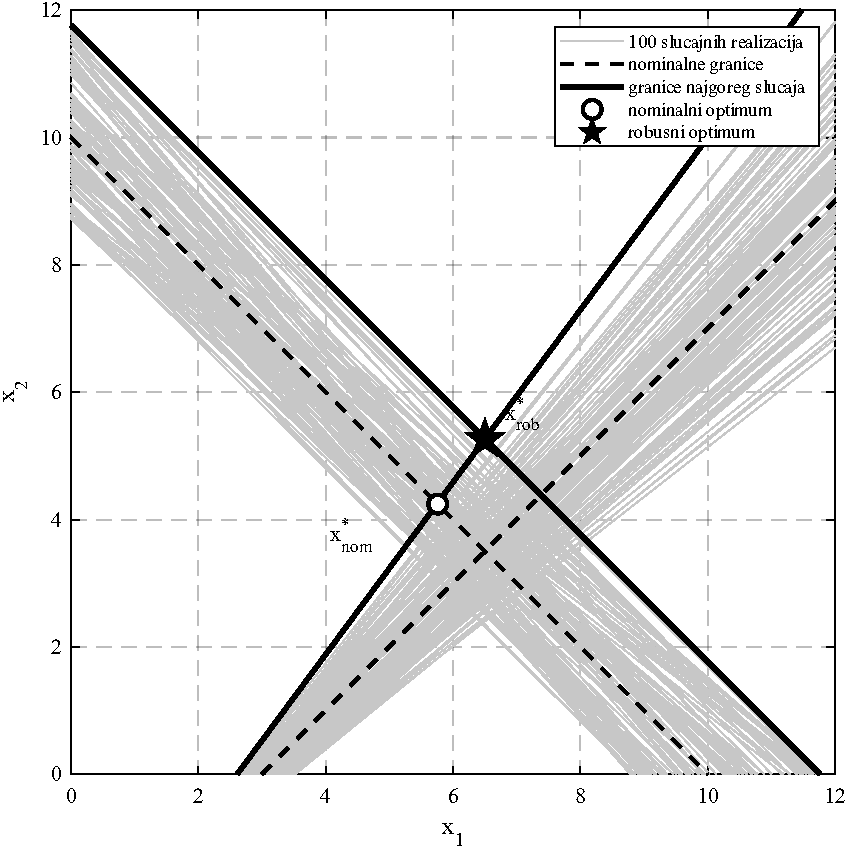
\includegraphics[width=0.88\linewidth]{../figures/fig2_1_robust_envelope_monte_carlo.pdf}
\caption{Granice ograničenja za 100 slučajnih realizacija koeficijenata (sivo),
nominalne granice (crtkano), granice najgoreg slučaja (puna crta) te nominalni i
robusni optimum (Slika 3.1 seminara v1.2).}
\label{fig:z2-realizacije}
\end{figure}

\subsection{Dekonstrukcija: svaki element slike posebno}

\begin{longtable}{@{}p{0.30\linewidth} p{0.66\linewidth}@{}}
\toprule
\textbf{Element} & \textbf{Što je i odakle dolazi} \\
\midrule
\endfirsthead
\toprule
\textbf{Element} & \textbf{Što je i odakle dolazi} \\
\midrule
\endhead
Osi $x_1$, $x_2$, raspon $0$--$12$ & Prostor projektnih varijabli, isti kao u
Zadatku 1, samo pomaknut u pozitivni kvadrant gdje leže oba rješenja. \\[5pt]
Snop tankih sivih pravaca & Rubovi ograničenja za $100$ slučajnih realizacija ---
dva pravca po realizaciji, dakle $200$ sivih linija. Snop koji ide od gore
lijevo prema dolje desno pripada prvom ograničenju, onaj od dolje lijevo prema
gore desno drugom. \\[5pt]
Debela crtkana crta & Nominalne granice, iz Zadatka 1: $x_1 + x_2 = 10$ i
$x_1 - x_2 = 3$. To je ,,sredina`` svakog snopa. \\[5pt]
Debela puna crta & Granice najgoreg slučaja, \eqref{eq:z2-wc1} i
\eqref{eq:z2-wc2}: $0{,}85(x_1+x_2) = 10$ i $1{,}15x_1 - 0{,}85x_2 = 3$. To je
\emph{omotnica} snopa --- svaka siva linija leži s njezine unutarnje strane. \\[5pt]
Prazan kružić, oznaka $x_{\mathrm{nom}}^{\star}$ & Nominalni optimum
$(5{,}758,\ 4{,}242)$. Leži \emph{unutar} snopa --- otprilike na polovini
njegove širine --- pa ga polovica realizacija izbacuje. \\[5pt]
Puna zvjezdica, oznaka $x_{\mathrm{rob}}^{\star}$ & Robusni optimum
$(6{,}500,\ 5{,}265)$, u sjecištu dviju punih crta, dakle na rubu \emph{omotnice}.
Nijedna siva linija ne prolazi između njega i dopustive strane. \\
\bottomrule
\end{longtable}

\begin{korak}[Što slika dokazuje --- i što ne]
\begin{enumerate}[leftmargin=*]
  \item \textbf{Zašto je nominalno rješenje krhko.} Kružić je usred snopa. Snop
        je gust upravo ondje, pa mala perturbacija koeficijenata pomiče granicu
        preko njega.
  \item \textbf{Zašto je robusno rješenje sigurno.} Zvjezdica je na sjecištu
        omotnica --- najbliža moguća točka nominalnom optimumu koja je s
        dopustive strane \emph{svake} sive linije istovremeno.
  \item \textbf{Koliko robusnost košta.} Udaljenost između kružića i zvjezdice je
        vizualna mjera cijene: robusno rješenje je dalje od središta nivo-elipsa,
        pa je funkcija cilja veća.
\end{enumerate}
\end{korak}

\begin{zamka}[Ograničenje ove slike, i što reći ako te pitaju]
Slika prikazuje \emph{rubove} dopustivih skupova, ne same skupove --- dopustive
strane nisu osjenčane. Uz $200$ sivih linija sjenčanje bi sliku učinilo
nečitljivom, pa je to svjesna odluka, ali se s crteža ne vidi izravno na kojoj je
strani svake linije dopustivo područje. Ako te se pita, reci upravo to i dodaj
orijentaciju: za prvo ograničenje dopustivo je \emph{iznad} pravca (veći
$x_1 + x_2$), za drugo \emph{iznad-lijevo} (manji $x_1 - x_2$), pa je dopustivi
presjek za svaku realizaciju klin koji se otvara prema gore desno --- kao u
Zadatku 1.
\end{zamka}

\section{Kako sliku nacrtati rukom}
\label{sec:z2-crtanje}

\begin{ploca}[Robusna slika, sedam poteza]
\begin{enumerate}[leftmargin=*]
  \item Osi $x_1$, $x_2$, raspon $0$ do $12$.
  \item Nominalni pravci crtkano: $x_1 + x_2 = 10$ i $x_1 - x_2 = 3$, kao u
        Zadatku 1.
  \item Uz svaki nominalni pravac nacrtaj po dvije-tri tanke linije s obje strane,
        blago zakrenute --- to predstavlja snop realizacija. Nemoj crtati sto
        linija; tri po strani prenose ideju.
  \item Debelo povuci omotnice: $x_1 + x_2 = 11{,}76$ (paralelno s nominalnim,
        pomaknuto prema gore desno) i $1{,}15x_1 - 0{,}85x_2 = 3$ (blago
        zakrenuto u odnosu na nominalni).
  \item Označi kružićem nominalni optimum $(5{,}76,\ 4{,}24)$ i naglasi da leži
        usred snopa.
  \item Označi zvjezdicom robusni optimum $(6{,}50,\ 5{,}26)$ u sjecištu debelih
        crta.
  \item Povuci strelicu od kružića do zvjezdice i uz nju napiši
        $\Delta f = +24{,}02$, odnosno $+39{,}6\%$ --- to je cijena robusnosti.
\end{enumerate}
\end{ploca}

\section{Usporedba s nominalnim rješenjem}
\label{sec:z2-usporedba}

\begin{seminar}{Seminar v1.2, Tablica 3.2 --- nominalno i robusno rješenje}
\begin{center}
\begin{tabular}{lccc}
\toprule
\textbf{Rješenje} & $x_1^*$ & $x_2^*$ & $f(x^*)$ \\
\midrule
Nominalno (Zadatak 1) & $5.757576$ & $4.242424$ & $60.606061$ \\
Robusno               & $6.500000$ & $5.264706$ & $84.623962$ \\
\midrule
Razlika               & $+0.742424$ & $+1.022282$ & $+24.017901$ ($+39.63\%$) \\
\bottomrule
\end{tabular}
\end{center}

Zahtjev za dopustivošću pri svim realizacijama sužava dopustivi skup i pomiče
optimum dalje od minimuma bez ograničenja, pa vrijednost funkcije cilja raste za
$24.017901$, odnosno $39.63\%$.
\end{seminar}

\begin{pojam}{Cijena robusnosti}
Razlika $f(x_{\mathrm{rob}}^{\star}) - f(\xopt) = 24{,}018$ je ono što se plaća
da rješenje ostane dopustivo pri \emph{svakoj} realizaciji, a ne samo pri
nominalnoj. Mehanizam je jednostavan: robusni dopustivi skup je podskup
nominalnoga (svaki robusno dopustiv $x$ zadovoljava i nominalnu realizaciju, jer
je i ona u skupu nesigurnosti), a minimum po manjem skupu ne može biti manji.
\end{pojam}

\section{Isti zaključak na predavanju}
\label{sec:z2-predavanje}

\begin{izvor}{Predavanje 8 --- Robusno optimiranje, slajd 8/21 (PDF str.~8)}
\slajd[0.78]{p08-primjer1-nominalno}

\textbf{Što je na slajdu.} Ilustracija \emph{nominalnog} rješenja profesorova
Primjera 1: dopustivi poliedar s četiri ograničenja i minimizator
$x^{\star} = (20,\ 10)$, koji leži u vrhu.
\end{izvor}

\begin{izvor}{Predavanje 8 --- Robusno optimiranje, slajd 9/21 (PDF str.~9)}
\slajd[0.78]{p08-primjer1-robusno}

\textbf{Što je na slajdu.} Isti problem s perturbiranim koeficijentima
($\pm 5\%$): minimizator se pomaknuo na $x^{\star} = (18{,}5714,\ 10)$.

\textbf{Isti obrazac kao kod nas:} robusni optimum je \emph{pomaknut u
unutrašnjost} u odnosu na nominalni, jer se dopustivi skup stegnuo. Kod
profesora se prva komponenta smanjila s $20$ na $18{,}57$; kod nas su se obje
povećale, jer nam ograničenja tjeraju rješenje prema gore desno. Smjer ovisi o
problemu --- ono što je uvijek isto jest da robusni optimum ne može biti bolji
od nominalnog.
\end{izvor}

\begin{izgovor}
,,Za grafički prikaz generirao sam sto slučajnih realizacija koeficijenata iz
zadanih intervala, uz fiksno sjeme generatora radi ponovljivosti. Za svaku sam
nacrtao oba rubna pravca, pa se dobiva snop.

Nominalni optimum leži usred tog snopa, i to zato što u Zadatku 1 leži točno na
granici prvog ograničenja. Očekivano je da ga otprilike polovica realizacija
izbaci iz dopustivog skupa --- u uzorku je to bilo pedeset četiri od sto.

Robusni optimum leži na sjecištu omotnica snopa, pa nijedna realizacija nije
prekršena. Naglasio bih da nula kršenja od sto nije dokaz robusnosti --- dokaz je
to što su zadovoljene sve četiri vršne nejednakosti po ograničenju, ukupno osam.
Realizacije samo ilustriraju.

Cijena robusnosti je porast funkcije cilja sa šezdeset zarez šest na osamdeset
četiri zarez šest dva, dakle trideset devet i pol posto. Razlog je što je
robusni dopustivi skup podskup nominalnoga, a minimum po manjem skupu ne može
biti manji.``
\end{izgovor}
